\NeedsTeXFormat{LaTeX2e}
\documentclass[12pt]{article}

\usepackage{titlesec}
\usepackage{setspace}
\usepackage{amsmath}
\usepackage{amssymb}
\usepackage{epsfig}
\usepackage{fancybox}
\usepackage{listings}
%\usepackage{algo}
\usepackage{url}
\usepackage{xcolor}
\usepackage{adjustbox}
\usepackage{float}
\usepackage{multicol}
\usepackage[utf8]{inputenc}
\usepackage[colorlinks=true,linkcolor=blue]{hyperref}

\newcommand{\phil}[1]{{\color{red}(\textbf{Phil:} #1)}}
\newcommand{\yue}[1]{{\color{blue}(\textbf{Yue:} #1)}}
\newcommand{\specialcell}[2][c]{%
	\begin{tabular}[#1]{@{}c@{}}#2\end{tabular}}


\setlength{\textheight}{9in}
\setlength{\textwidth}{6in}
\setlength{\oddsidemargin}{.25in}
\setlength{\topmargin}{-.5in}  % changed from -.25 by RSR on 1/21/07
%\parindent .5in    % commented out by RSR 1/21/07

\hyphenation{itself}
\setcounter{secnumdepth}{4}
\setcounter{tocdepth}{4}
%%%%%
%% Commented out -- RSR, 1/21/07
%%%%%
% The following provides a box to surround the thesis statement
\newenvironment{Thesis}%
{\begin{Sbox}\begin{minipage}{.95\linewidth}}%
		{\end{minipage}\end{Sbox}\begin{center}\fbox{\TheSbox}\end{center}}

\title{Stream Mining Algorithms for Sensor Data Classification}
\author{
    Yue Dong\\
	\texttt{yuedong029@uottawa.ca}
	\and
	Philippe Paradis\\
	\texttt{philippe.paradis@carleton.ca}
}

\begin{document}
\singlespace
\maketitle

\tableofcontents
\newpage
\section*{Acknowledgements}


\begin{abstract}                % ~350 words max


\end{abstract}

% This sets section-numbering to only include Section and Subsection numbers
\setcounter{secnumdepth}{4}

\section{Introduction}
\label{sec:introduction}

\section{Dataset \& Data exploration}
\subsection{Dataset}
The dataset we used is the Bike Sharing Dataset from the UCI repository. Ac coding to the dataset description, ``this dataset contains the hourly and daily count of rental bikes between years 2011 and 2012 in Capital bikeshare system with the corresponding weather and seasonal information.''
 The summary of this dataset is as Table \ref{table:dataset} shows. More information of the dataset can be found at \url{http://archive.ics.uci.edu/ml/datasets/Bike+Sharing+Dataset}.
 
\begin{table}[H]
	\label{table:dataset}
	\begin{tabular}{| l | p{11cm} |} \hline
		Number of instances: & 17389 (hours), 731 (days)\\
		Number of Attributes: & 16\\ \hline \hline
		\textbf{Attributes details:} &\\ \hline
		Attribute name  & description\\ \hline
		instant   & record index\\ \hline
		dteday    & date\\ \hline
		season  & season (1:springer, 2:summer, 3:fall, 4:winter)\\ \hline
		yr    &  year (0: 2011, 1:2012)\\ \hline
		mnth &   month ( 1 to 12)\\ \hline
		hr & hour (0 to 23) \\ \hline
		holiday   & weather day is holiday or not \\ \hline
		weekday   &  day of the week \\ \hline
		workingday   & 1: if day is neither weekend nor holiday; 0: otherwise.\\ \hline
		weathersit   & 1: Clear; 2: Mist; 3: Light Snow, Light Rain; 4: Heavy Rain, Ice Pallets, Snow + Fog;\\ \hline
		temp   & Normalized temperature in Celsius. \\ \hline
		atemp    & Normalized feeling temperature in Celsius. \\ \hline
		windspeed   & Normalized wind speed. \\ \hline
		casual   & count of casual users\\ \hline
		registered   & count of registered users\\ \hline
		cnt   & count of total rental bikes including both casual and registered \\ \hline
	\end{tabular}
	\caption{Bike sharing dataset summary}
\end{table}
 
 
\section{Data Visualization}
\label{sec:visual}
 
What relationships do we expect to see in the data?
\begin{itemize}
	\item Variation in bike rentals based on hour of the day
	\item Different bike rental patterns on the weekends versus regular weekdays
	\item Different  bike rental patterns on holidays versus non-holidays
	\item Variation in bike rentals based on temperature
	\item Variation in bike rentals based on weather condition
	\item No idea about effects of humidity
	\item Variation in bike rentals based on wind speed
\end{itemize}

What kind of relationships do we expect to see in the data?
\begin{itemize}
	\item On regular weekdays, spike in traffic during morning and afternoon rush hours
	\item Typically, higher bike rental volumes during the day and lower during the night
	\item In other words, highly non-linear relationship between bike rentals and datetime
	\item Roughly linear variation between bike rentals and temperature (although very high summer temperatures could lead to reduced bike rental volumes)
	\item 
\end{itemize}
 
\subsection{Missing values}

- What could possibly explains the missing values that we see?
There is clearly a pattern in the missing values. Most of those happen at the same time at night.
Also, the bike count values tend to change and be much smaller around missing values. Why is that?


\begin{figure}[H]
	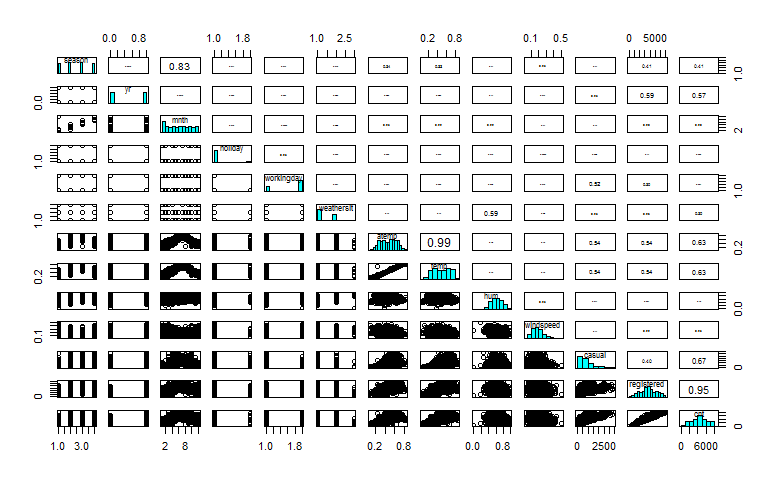
\includegraphics[scale=0.6]{figures/scatterplot.png}
	\label{fig:scatterplot}
	\caption{Scatterplot matrix of bike sharing (daily) dataset}
\end{figure}

As we can see from Figure \ref{fig:scatterplot}, there are 0.83 correlation between season and mnth, 0.99 correlation between temp and atemp, and 0.95 correlation between registered and cnt, 0.67 between casual and cnt.

High correlation between two variables means that as one variable rises or falls, the other variable rises or falls as well. Since we don't want high correlation in our dataset, we can drop month, and atemp.

Moreover, from observing the last three columns of correlation between different attributes to registered, casual, and cnt, we can have a list of the correlations in decreasing order as the following table shows: 
\begin{table}[H]
	\begin{tabular}{| l | l | l | l | l | l|}
		cnt~ & registered & casual & temp/atemp & yr & season\\
		correlation & 0.95 & 0.67 & 0.63 & 0.57 & 0.41\\
		\hline
	%	registered~ &
	\end{tabular}
\end{table}
Random sampling 1000 instances without replacement, and draw the scatterplot matrix shows that the hours have a high correlation with the hourly cnt. 
\begin{figure}[H]
	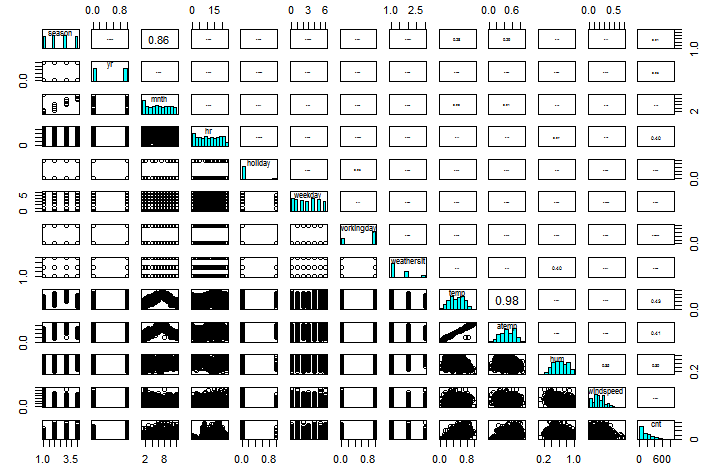
\includegraphics[scale=0.8]{figures/scatterplot_col_season.png}
	\end{figure}

Therefore, we identify that temp, yr, season/mth, hr, and workingday as our main focus.

1. Most likely, temperature and weather have correlation with bike demand. We can plot:

Explore 2. Most certain the hour of the day also correlates with Bike demand 

Explore 3. Finally let’s see if usage varies depending on the month 

In short we have identified strong correlation with these predictors: 1. Temperature 2. Hour of the Day 3. Working Day 4. Month of the Year

\subsection{Association Rule Mining}
From the data visualization, there is one unanswered question left: How can we know where the PEAK rental periods are on an overall basis?

To find more about this, we did an association rule mining. The bike sharing dataset contains a mixture of categorical and numeric attributes and therefore need some preparation before using apriori algorithm on it.

temp : Normalized temperature in Celsius. The values are divided to 41 (max)
- atemp: Normalized feeling temperature in Celsius. The values are divided to 50 (max)
- hum: Normalized humidity. The values are divided to 100 (max)
- windspeed: Normalized wind speed. The values are divided to 67 (max)

\section{Unsupervised Learning: Data Preprocessing}
\subsection{Dimension Reduction: PCA }
\label{sec:dimension-reduction}

\subsection{Data Reduction: Clustering kmeans+Davies-Bouldi index}
\label{data-reduction}

The bike sharing dataset has  17365 data instances for the hourly bike sharing dataset. Instead of dimension reduction to reduce the number of attributes, we can use data reduction to reduce the number of cases. In this section, we consider to use clustering methods to cluster together similar cases and also try unsupervised learning for outlier detection. By doing so, we can have a reduced representation in volume but produces the same or similar analytical results.
\subsubsection{Fill in missing values}
Data cleaning, smooth noisy data, identify or remove outliers, and resolve inconsistencies
\subsubsection{Data transformation}

\subsection{Data Reduction: Outlier Detection}






\section{Experimental Design}
\label{sec:experimental-design}


\section{Supervised Learning}

The most obvious supervised learning task is to predict \texttt{cnt}, which is a regression problem, since \texttt{cnt} is a continuous variable. This has practical applications, as any company managing a bicycle sharing system might be interested in having a predictive models that helps ensure the supply of bicycles is always appropriate.

\subsection{Kaggle Competition}

The UCI Bike Sharing Dataset is featured as a Kaggle problem called \emph{Bike Sharing Demand}\footnote{\url{www.kaggle.com/c/bike-sharing-demand}}. We decided to participate in the competition, so that we could compare the performance of our method with others.

The competition started on 28 May 2014 and ends on 29 May 2015. As of 13 April 2015, approximately 2900 people or team have participated in this competition, submitting more than 26000 entries.

The Bike Sharing dataset provided by Kaggle is essentially the same as UCI's -- there are only minor differences in the format, such as the date and hour being specified by only one column named \texttt{datetime} and non-normalized units used for temperature, humidity and wind speed.

The data must be split into a training set and a testing set, where the training set is comprised of the first 19 days of every month and the testing set is comprised of the 20th day until the end of the month.

The objective of the competition is to train a classifier on the training data and to predict the testing data's \texttt{cnt} field with the lowest possible root-mean-squared-logarithmic error (RMSLE).

Users can submit their predictions online and the RMSLE will be calculated

Note that the testing data on Kaggle excludes the \texttt{cnt} field. As such, users must submit their predictions only to discover its RMSLE. However, the full data is present in the UCI's dataset and so, we can compute the RMSLE of our predictions by ourselves.

\section{Data preparation}
WILL MOST LIKELY NEED TO MOVE THIS SOMEWHERE ELSE AND JUST REFER TO IT HERE.

The relationship between \texttt{atemp} and \texttt{cnt} is non-linear, as can be seen from GRAPHREF. However, there seems to be a peak temperature for bike rentals at around PEAKTEMP. Hence, it would make sense to define a new variable corresponding to the (absolute value) difference between the current temperature and this ``ideal temperature''. Let \texttt{atempdiff} be defined as:
\begin{verbatim}
atempdiff <- abs(atemp - PEAKTEMP)
\end{verbatim}
Then, the relationship between \texttt{atemptdiff} and \texttt{cnt} is roughly linear as we can see from OTHERGRAPH.

\section{Supervised Learning}
\label{supervised learning}

\subsection{The two alternative problems on Kaggle}

Unfortunately, the problem of modeling and predicting bike rental demand as stated on Kaggle as two different interpretations.

\begin{enumerate}
	\item Imputation of missing values.
	\item Predictive modeling.
\end{enumerate}

The first problem of imputation is more popular on Kaggle and 

\section{Experiments and Results}
\label{sec:experiments-and-results}

\section{Kaggle Competition}




\section{Conclusion and Further Work}
\label{sec:conclusion}



\begin{thebibliography}{9}
\bibitem{dataset}
Fanaee-T, Hadi, and Gama, Joao, 'Event labeling combining ensemble detectors and background knowledge', Progress in Artificial Intelligence (2013): pp. 1-15, Springer Berlin Heidelberg.
\end{thebibliography}

\end{document}
